\chapter{Аналитический раздел}
В указанной постановке задача не решалась, однако можно очертить некоторые этапы, которые так или иначе должны присутствовать в решении задачи:
\begin{itemize}
    \item Сбор новостей из открытых информационных источников;
    \item Кластеризация новостей по сюжетам;
    \item Ранжирование источников.
\end{itemize}

Перед анализом существующих методов каждого из этапов рассмотрим сущности предметной области (рис.~\ref{fig:domain}):
\begin{itemize}
    \item Источники~--- поставщики новостей, идентифицируются адресом;
    \item Лента~--- новостные ленты, содержащие список новостей за последнее время, предоставляются источниками;
    \item Новость~--- непосредственно текст новости, опубликованной источником;
    \item Сюжет~--- объединение различных новостей, относящихся к одному и тому же событию.
\end{itemize}

\begin{figure}[h]
    \centering
    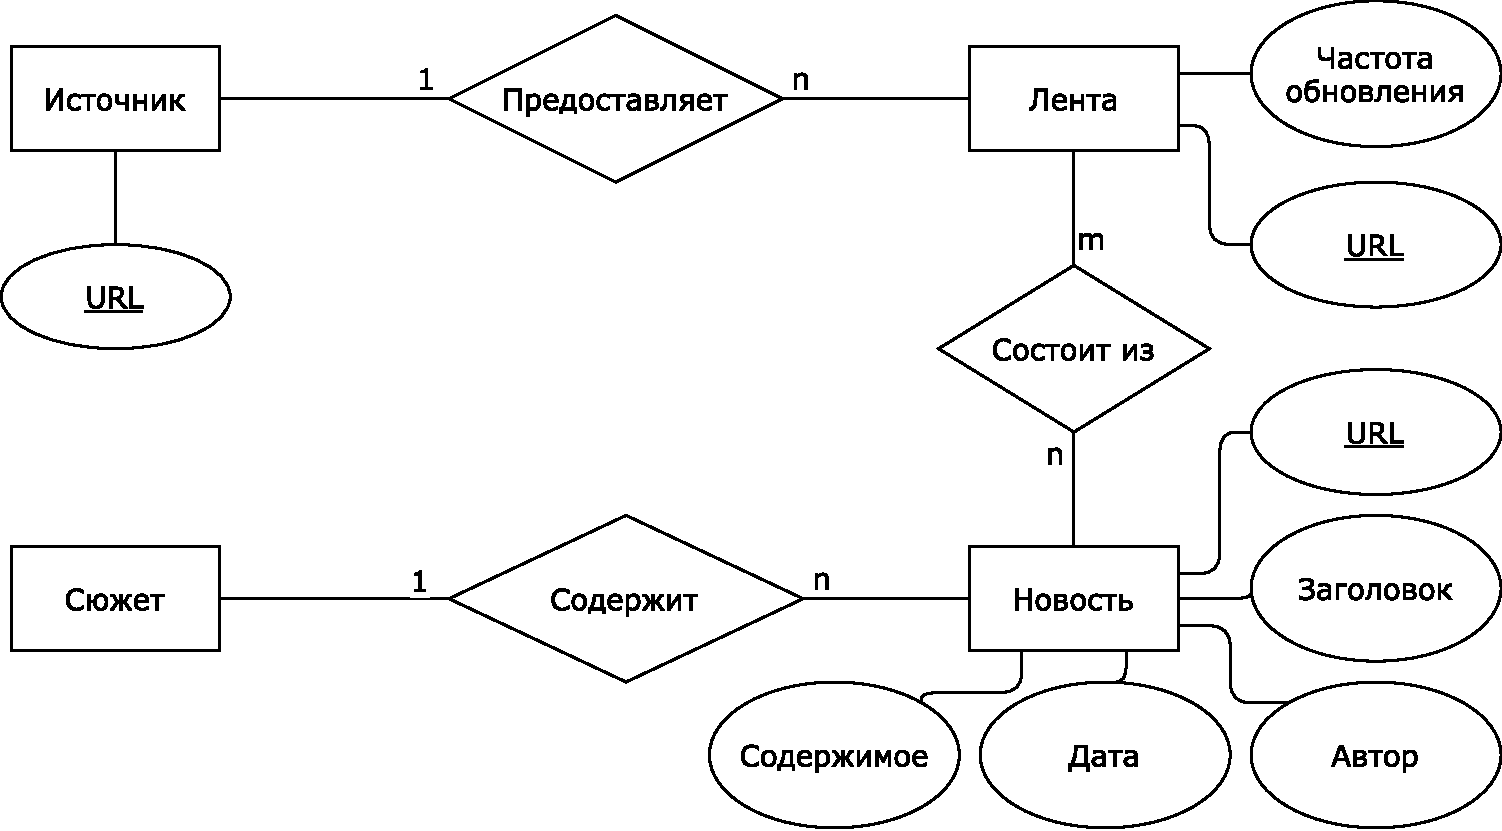
\includegraphics[width=\textwidth]{domain.pdf}
    \caption{Сущности предметной области.}
    \label{fig:domain}
\end{figure}

\section{Сбор новостей} \label{sec:collecting}
Сбор актуальных новостей является важной задачей в разрабатываемой системе, потому что качество и актуальность собранной информации влияет на выделение сюжетов, что, в свою очередь, виляет на ранжирование источников.

С данной задачей связано большое количество проблем: огромное число новостных источников, ограничительная пропускная способность каналов, зашумлённость страниц второстепенной информацией и так далее.

\subsection{Новостные ленты}
Большинство новостных источников, включая новостные сайты и популярные группы в социальных сетях, предоставляют rss- и atom- ленты~--- небольшие xml-документы, в которых описываются последние новости и ссылки на них. Такие ленты стараются поддерживать актуальными, поскольку они используются многими новостными агрегаторами, которые активно используются пользователями.

Важно отметить, что в самих лентах не хранится непосредственно текст новостей, а лишь ссылки на html-страницы, расположенные на сайте источников, поэтому после получения ленты необходимо выгружать страницы с сайта источника.

\subsection{Фильтрация посещённых страниц}
Один источник может предоставлять несколько лент, например по ленте на категорию или тематику. Поэтому одна и та же новость может быть получена из нескольких лент, что будет создавать дополнительную нагрузку на систему. Поэтому имеет смысл отбрасывать уже посещённые новостные страницы. Очевидное на первый взгляд решение проблемы~--- использование ассоциативных массивов~--- довольно требовательно к памяти, поэтому имеет смысл рассмотреть использование вероятностных фильтров. Наиболее популярным фильтром подобного рода является фильтр Блума.

\subsubsection{Фильтр Блума} \label{sssec:bloom-filter}
Фильтр Блума~--- вероятностная структура данных, позволяющая компактно хранить множество элементов и проверять принадлежность заданного элемента к множеству \cite{bloom70}. При этом существует вероятность получить ложноположительный результат, то есть ситуацию, когда элемента в множестве нет, но фильтр сообщает, что элемент есть.

Фильтр Блума может использовать любой объём памяти, заранее заданный пользователем, причём чем он больше, тем меньше вероятность ложного срабатывания. Поддерживается операция добавления новых элементов в множество, но не удаления существующих (если только не используется модификация со счётчиками).

\begin{figure}[h]
    \centering
    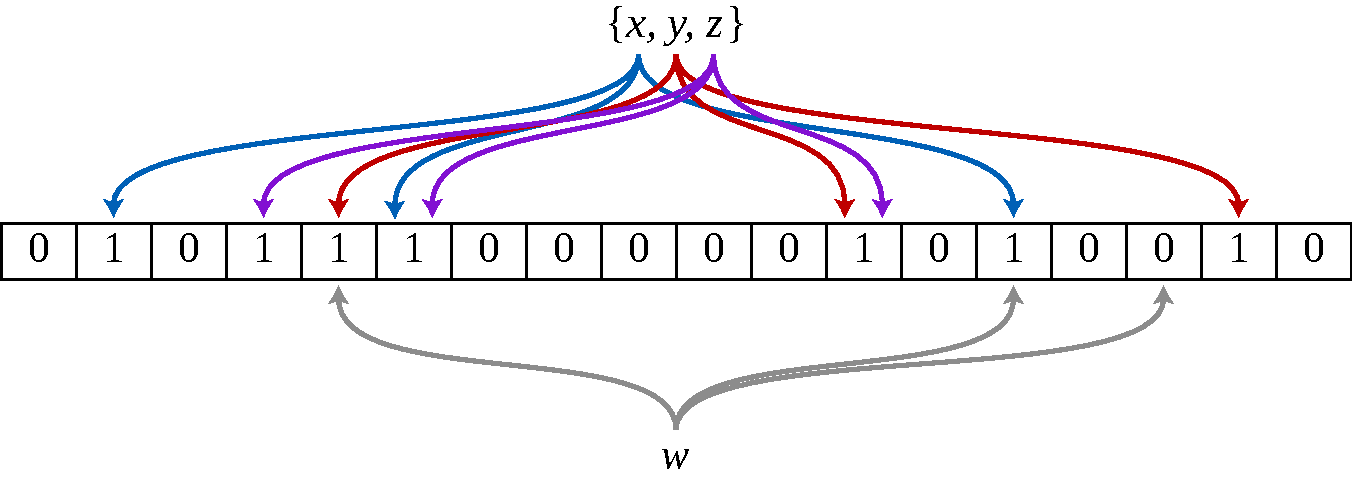
\includegraphics[width=\textwidth]{bloom-filter.pdf}
    \caption{Пример фильтра Блума с $m=18$ и $k=3$.}
\end{figure}

Фильтр Блума представляет собой битовый массив из $m$ бит. Изначально, когда структура данных хранит пустое множество, все $m$ бит обнулены. После чего определяются $k$ независимых хеш-функций $h_i$, отображающих каждый элемент в одну из $m$ позиций битового массива достаточно равномерным образом.

Для добавления элемента $e$ необходимо записать единицы на каждую из позиций $h_i(e)$ битового массива.

Для проверки принадлежности элемента $e$ к множеству хранимых элементов, необходимо проверить состояние битов $h_i$. Если хотя бы один из них равен нулю, элемент не может принадлежать множеству (иначе бы при его добавлении все эти биты были установлены). Если все они равны единице, то структура данных сообщает, что $e$ принадлежит множеству. При этом может возникнуть две ситуации: либо элемент действительно принадлежит к множеству, либо все эти биты оказались установлены по случайности при добавлении других элементов, что и является источником ложных срабатываний в этой структуре данных.

Согласно \cite{broder02}, для заданных $n$~--- числа ожидаемых элементов в множестве и $p$~--- максимальной вероятности ложноположительного срабатывания возможно вычислить оптимальный размер $m$ как
\begin{equation}
    m=-\frac{n\ln p}{(\ln 2)^2},
\end{equation}
и оптимальное количество хеш-функций как
\begin{equation}
    k=\frac{m}{n}\ln 2.
\end{equation}

\subsection{Стандарт исключений для роботов} \label{ssec:robotstxt}
Следующая проблема, возникающая во время сбора новостей, заключается в том, что после получения новостной ленты нам необходимо сделать множество запросов к одному серверу, что обычно не нравится владельцам сайтов.

Для уменьшения нагрузки на сервера владельцы сайтов ограничивают доступ к определённым страницам для ботов, используя для этого файл \verb|robots.txt|, находящийся в корне сайта (то есть по пути \verb|/robots.txt|). Это может быть полезно для ограничения частоты запросов со стороны роботов, запрета индексирования динамический и служебных страниц. Несоблюдение указанных в файле ограничений ведёт к блокировке доступа для робота.

Формат файла имеет следующий вид:
\begin{verbatim}
<поле>:<необязательный пробел><значение><необязательный пробел>
\end{verbatim}

Стоит заметить, что вместо пробела могут использоваться также другие пробельные символы, а \verb|поле| является регистронезависимым.

Основные используемые поля:
\begin{itemize}
    \item \verb|user-agent|: стандартное поле, используется для задания имени бота, которому адресованы последующие правила, либо \verb|*|, если всем;
    \item \verb|disallow|: стандартное поле, используется для задания пути, индексация которого запрещена. В пути разрешены два спец-символа: \verb|*| (любое количество любых символов) и \verb|$| (конец пути). Причём путь, к примеру, \verb|/path/to/file| действует аналогично \verb|/path/to/file*|;
    \item \verb|crawl-delay|: нестандартное поле, используется для задания минимальной задержки в секундах между запросами со стороны робота.
\end{itemize}

Наличие данного файла и ограничения, указанные в нём, необходимо учитывать при загрузке новостей, чтобы система не была заблокирована владельцами сайта.

\subsection{Разбор страницы}
Далеко не вся информация на странице ценна для поставленной задачи. Например, информация, размещённая в подвале и по сторонам страницы несёт обычно служебную информацию, которая может быть полезна при обходе страниц (так как может содержать полезные ссылки), но бесполезна конечному пользователю и не содержит информации, относящейся к новости. Поэтому ставится задача выделения основного содержимого, то есть непосредственно текста новости, из html-страницы. Для этого необходимы методы выделения такой информации, которые в основном базируются на эвристиках и применимы для большинства страниц \cite{pomikalek11}.

\subsubsection{Выделение основного содержимого} \label{sssec:readability}
Для получения основного содержимого во многих случаях достаточно сохранять только текстовые элементы HTML, то есть блоки текста, которые не прерывались разметкой, которые имеют более чем десяток слов. Текст на страницах принадлежит к одному из двух типов, в зависимости от назначения: <<навигационного>> и <<информационного>>.

Для элементов навигации обычно применяется текст, состоящий из нескольких слов (например, <<STOP>>, <<Прочтите это>>, <<Нажмите здесь>>), в то время как для основного содержимого используется много слов.

В то время как это разделение работает во множестве случаев, все становится сложнее с заголовками, короткими предложениями, отказами от ответственности, авторскими правами и другими колонтитулами.

Есть более сложные стратегии, а также функции, которые помогают отделять основное содержание от шаблонного \cite{kohlschutter10}:
\begin{enumerate}
    \item Рассмотренная выше плотность HTML-тегов;
    \item Ссылочная плотность (количество слов внутри ссылок по сравнению с общим количеством слов в блоке);
    \item Текстовые характеристики: количество запятых, длина текста и другие;
    \item Связь текущего блока с контекстом (с предыдущими и следующими блоками);
    \item Семантическая DOM-структура документа (\verb|<article>|, \verb|<section>| и другие);
    \item Визуальное изображение страницы (например, большие изображения, окружённые текстом);
\end{enumerate}

Результирующий алгоритм, используя комбинацию этих факторов, рекурсивно оценивает все узлы документа, находя наиболее похожие на основное содержимое.

\subsubsection{Декодирование мнемоник HTML} \label{sssec:html-mnemonics}
Мнемоника~--- это конструкция SGML, которая ссылается на символ из набора символов текстового файла. В HTML предопределено большое количество спецсимволов. Чтобы вставить определённый символ в разметку, нужно вставить определенную ссылку-мнемонику в HTML-структуру.

Мнемоника имеет вид \verb|&...;|. Так, например, буква <<q>> может представляться как \verb|&#113;|, а <<--->> как \verb|&mdash;|.

\subsubsection{URL нормализация} \label{sssec:url-normalization}
Различные URL могут указывать на одну и ту же страницу, но отличаться при этом незначительно.

URL нормализация~--- процесс приведения URL к каноничному виду, путём применения различных правил трансляции адресов. Не все правила дают строго эквивалентные URL, поэтому выделяют два типа нормализации \cite{pant04}:
\begin{itemize}
    \item Безопасная нормализация, в результате которой URL указывает на ту же страницу;
    \item Агрессивная нормализация, в результате которой URL чаще всего указывает на несуществующую страницу.
\end{itemize}

Ключ страницы~--- своего рода хеш, получаемый в результате агрессивной нормализации, то есть применения всех правил, указанных в данном разделе. Ключ страницы может служит идентификатором новости, ленты и источника.

Относительно безопасные преобразования:
\begin{enumerate}
    \item Конвертация в нижний регистр компонентов схемы и хоста: \\ \verb|HTTP://www.Example.com/| в \verb|http://www.example.com/|;
    \item Удаление относительных каталогов, сегментов-точек: \\ \verb|http://example.com/../a/b/../c/./d| в \verb|http://example.com/a/c/d|;
    \item Удаление фрагментов: \\ \verb|http://example.com/bar.html#section1| в \verb|http://example.com/bar.html|;
    \item Удаление конечного слеша: \\ \verb|http://example.com/foo/| в \verb|https://example.com/foo|;
    \item Удаление порта по умолчанию: 80 для http и 443 для https \\ \verb|http://example.com:80| в \verb|http://example.com|;
    \item Перевод IDN в unicode: \\ \verb|http://xn--e1afmkfd.xn--80akhbyknj4f/| в \verb|http://пример.испытание/|.
\end{enumerate}

Преобразования, которые можно использовать для проверки эквивалентности двух страниц, но не при запросе:
\begin{enumerate}
    \item Удаление головного индекса (\verb|index.html|, \verb|default.aspx| и другие): \\ \verb|http://example.com/index.html| в \verb|http://www.example.com/|;
    \item Удаление дублированных слешей: \\ \verb|http://example.com/foo//bar.html| в \verb|http://example.com/foo/bar.html|;
    \item Удаление \verb|www.|: \\ \verb|http://www.example.com/| в \verb|http://example.com/|;
    \item Сокращение идентификаторов протокола: \\ \verb|https://example.com| в \verb|http://example.com|;
    \item Конвертация в нижний регистр всего URL: \\ \verb|HTTP://example.COM/TEST.html| в \verb|http://example.com/test.html|;
\end{enumerate}

Такие преобразование применимы для построения ключа страницы, но не для упрощения адреса ссылки.

\section{Кластеризация новостей}
\subsection{Векторное представление новости} \label{ssec:vectorization}
Чтобы иметь возможность группировать новости по сюжетами нам необходим метод, позволяющий сравнивать новостные документы. К сожалению, две новости не могут сравниваться непосредственно, но могут быть представлены в векторной форме, допускающей такие сравнения.

Наиболее популярной формой такого представления является представление <<мешком слов>>~--- то есть вектором $\vect{x}$, где каждая компонента соответствует определённому слову, входящему в данную новость $x$ \cite{frakes92}.

Однако же у такой модели есть недостаток: представляя текст как <<мешок слов>>, мы теряем контекст. Например, документы <<кролик быстрее, чем черепаха>> и <<черепаха быстрее, чем кролик>> имеют одинаковое векторное представление.

Простейшей характеристикой слова, которую можно использовать в данном представлении, является частота вхождения слова (от англ. TF~--- term frequency) в новость:
\begin{equation} \label{eq:tf}
    tf_{w,x}=\frac{n_{w,x}}{|x|},
\end{equation}
\begin{conditions}
    $|x|$ & длина новости $x$ (количество слов в ней); \\
    $n_{w,x}$ & количество вхождений слова $w$ в новость $x$. \\
\end{conditions}

Однако данная характеристика обладает существенным недостатком: популярные слова имеют больший вес по сравнению с менее популярными словами, что понижает качество кластеризации. Для решения этой проблемы вводят обратную частоту документа.

Обратная частота документа (от англ. IDF~--- inverse document frequency)~--- инверсия частоты, с которой слово встречается в документах. Учёт IDF уменьшает вес широкоупотребительных слов.
\begin{equation} \label{eq:idf}
    idf_w=\log\frac{N}{N_w},
\end{equation}
\begin{conditions}
    $N$ & количество новостей в коллекции;\\
    $N_w$ & количество новостей, содержащих слово $w$, $N_w=|\{x: x\ni w\}|$.
\end{conditions}

Объединяя (\ref{eq:tf}) и (\ref{eq:idf}), получаем TF-IDF характеристику:
\begin{equation} \label{eq:tf-idf}
    tf\text{-}idf_{w,x}=tf_{w,x}\cdot idf_w
\end{equation}

Векторное представление для новости $x$ в данном случае принимает вид:
\begin{equation}
    \vect{x}=(tf\text{-}idf_{w_1,x}, \quad tf\text{-}idf_{w_2,x}, \quad ...)
\end{equation}

Теперь вес некоторого слова пропорционален количеству употребления этого слова в новости, и обратно пропорционален частоте употребления слова в других новостях коллекции.

\subsection{Предобработка}
\subsubsection{Стоп-слова}
Существование заведомо высокочастотных слов (таких как <<an>>, <<and>>, <<и>>, <<как>> и др.) ведёт к раздуванию векторного представления. При этом вклад таких слов в семантику новости минимален и не влияет на кластеризацию по сюжетам. Поэтому разумно фильтровать данные слова при переводе новости в соответствующую векторную форму.

\subsubsection{Лемматизация и стемминг} \label{sssec:stemming}
При построении векторного представления в виде <<мешка слов>> нет смысла различать формы (склонения, спряжения) одного и того же слова. Это приведёт к неоправданному разрастанию словаря, дроблению статистики, увеличению ресурсоёмкости и снижению качества модели кластеризации.

\emph{Лемматизация}~--- это приведение каждого слова в документе к его нормальной форме. В русском языке нормальными формами считаются: для существительных~--- именительный падеж, единственное число; для прилагательных~--- именительный падеж, единственное число, мужской род; для глаголов, причастий, деепричастий~--- глагол в инфинитиве.

\emph{Стемминг}~--- это более простая технология, которая состоит в отбрасывании изменяемых частей слов, главным образом, окончаний. Она не требует хранения словаря всех слов и основана на правилах морфологии языка. Недостатком стемминга является большее число ошибок.

\subsection{Меры схожести новостей} \label{ssec:similarity}
\subsubsection{Эвклидова метрика}
Эвклидова метрика~--- <<классическое>> расстояние между двумя точками в пространстве \cite{huang08}:

\begin{equation}
    d(\vect{x},\vect{y})=\sqrt{\sum_{i=1}^n(x_i-y_i)^2},
\end{equation}
где $n$~--- размерность пространства.

Эвклидова метрика является наиболее просто мерой сходства между двумя векторами, однако плохо себя показывает относительно других мер при работе с текстами \cite{strehl00} и требует вычисления квадратного корня.

\subsubsection{Косинусная мера}
Косинусная мера основана предположении о том, что направление векторов имеет большее значение, чем длина каждого вектора и расстояние между ними \cite{zhong05}.

Данный метод, как следует из названия, основывается на косинусе угла между векторами:
\begin{equation}
    sim_c(\vect{x},\vect{y})=\frac{\vect{x}\cdot\vect{y}}{\lVert\vect{x}\rVert\lVert\vect{y}\rVert}
\end{equation}

\begin{figure}[h]
    \centering
    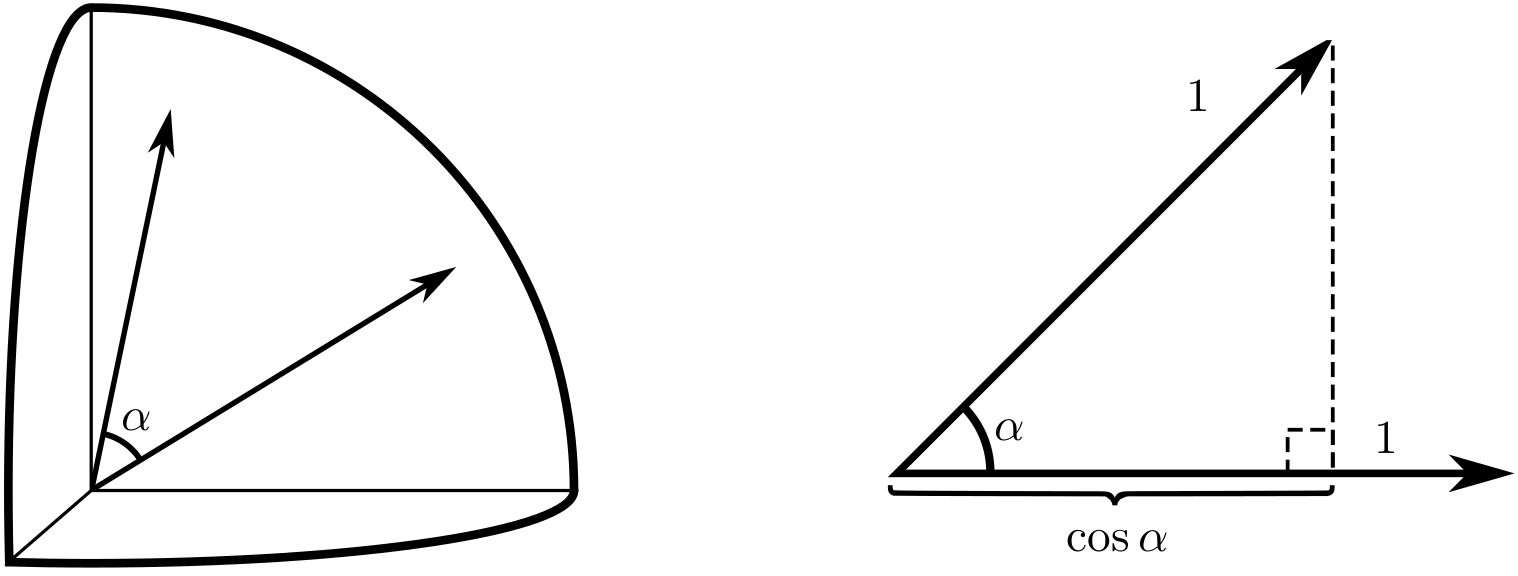
\includegraphics[width=.7\textwidth]{cosine.png}
    \caption{Косинусная мера двух единичных векторов.}
\end{figure}

В качестве длины вектора берётся эвклидова норма:
\begin{equation}
    \lVert\vect{x}\rVert=\sqrt{\vect{x}\cdot\vect{x}}
\end{equation}

Так как компоненты векторов неотрицательны исходя из выбранного представления, то значение данной меры лежит в диапазоне $[0,1]$, где значение $1$ указывает на одинаковое направление векторов, а $0$ на отсутствие общих слов.

Так как в данной мере используется только направление векторов, то достаточно работать с единичными векторами:
\begin{equation}
    \vect{\hat{x}}=\frac{\vect{x}}{\lVert\vect{x}\rVert}
\end{equation}

Таким образом, приходим к нормализованной версии косинусной меры:
\begin{equation}
    sim_c(\vect{\hat{x}},\vect{\hat{y}})=\vect{\hat{x}}\cdot\vect{\hat{y}}
\end{equation}

Что даёт возможность сильно упростить вычисления.

\subsubsection{Мера Жаккара}
Для лучшего понимания меры Жаккара сначала рассмотрим бинарный коэффициент Жаккара \cite{strehl02}:
\begin{equation}
    sim_{bj}=\frac{|S_x\cap S_y|}{|S_x\cup S_y|},
\end{equation}
где $S_x$ и $S_y$~--- множество слов в документе $x$ и $y$ соответственно.

Мера Жаккара определяется аналогично бинарному коэффициенту для случаев, когда вектора имеют не бинарные компоненты, а неотрицательные действительные значения \cite{manning09}:
\begin{equation}
    sim_j(\vect{x},\vect{y})=\frac{\vect{x}\cdot\vect{y}}{\lVert\vect{x}\rVert^2 + \lVert\vect{y}\rVert^2-\vect{x}\cdot\vect{y}}
\end{equation}

Данная мера показывает вес пересекающихся слов из обоих документов против веса слов, представленных только в одном из двух документов.

Мера Жаккара, аналогично косинусной мере, принимает значение в диапазоне $[0,1]$, где $1$ означает идентичность векторов.

\subsubsection{Эвристики}
В контексте задачи объединения новостей в сюжеты могут быть применены некоторые эвристики, влияющие на определение схожести новостей.

Во-первых, редко, когда новостной источник публикует две или больше новостей об одном и том же событии со схожей информацией, то есть фактически дублирует новость. Основываясь на данном предположении, можно добавлять штраф к схожести двух новостей от одного источника.

Во-вторых, новостные источники стараются максимально быстро опубликовать новость после соответствующего события, поэтому новости, образующие сюжет, публикуются приблизительно в одно время. Из этого следует, что имеет смысл добавлять штраф к схожести новостей пропорционально времени между ними.

Теперь штраф можно использовать с любой мерой схожести:
\begin{equation}
    sim'(x,y)=sim(\vect{x},\vect{y})\cdot(1-penalty(x,y)),
\end{equation}
\begin{conditions}
    $sim(\cdot,\cdot)$ & мера схожести в диапазоне $[0,1]$; \\
    $penalty(\cdot,\cdot)$ & суммарный штраф в диапазоне $[0,1]$. \\
\end{conditions}

\subsection{Меры схожести кластеров}
Во многих алгоритмах кластеризации предполагается объединение нескольких кластеров в один. Для этого необходимо ввести меру схожести кластеров.

\subsubsection{По ближайшему соседу}
\begin{figure}[h]
    \centering
    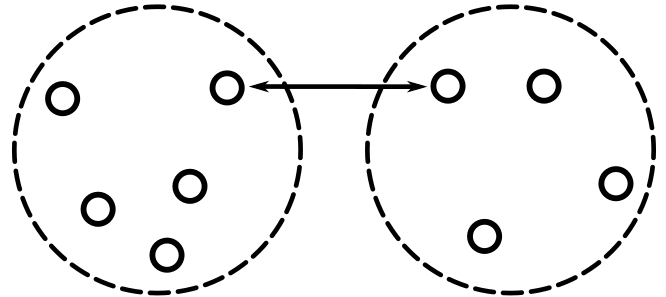
\includegraphics[width=.7\textwidth]{single-link.png}
    \caption{Мера схожести кластеров по ближайшему соседу.}
\end{figure}

Схожесть кластеров определяется как схожесть наиболее близкой пары новостей:
\begin{equation}
    sim_{near}(C_i,C_j)=\max_{x\in C_i,y\in C_j}sim(\vect{x},\vect{y}),
\end{equation}

Однако данная мера обладает существенным недостатком: создаётся цепочка связанных кластеров, каждая связанная пара который схожа по данной мере, в отличие от крайних кластеров:
\begin{figure}[h]
    \centering
    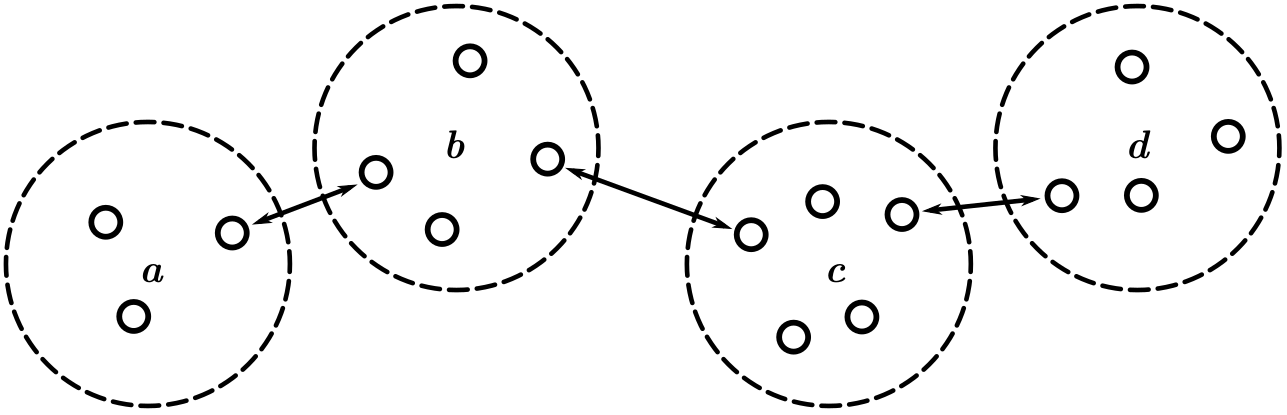
\includegraphics[width=\textwidth]{single-link-chain.png}
    \caption{Цепочка схожих кластеров.}
\end{figure}

\subsubsection{По дальнему соседу}
Аналогичным образом определяется мера по самому дальнему соседу:
\begin{equation}
    sim_{far}(C_i,C_j)=\min_{x\in C_i,y\in C_j}sim(\vect{x},\vect{y}),
\end{equation}

\begin{figure}[h]
    \centering
    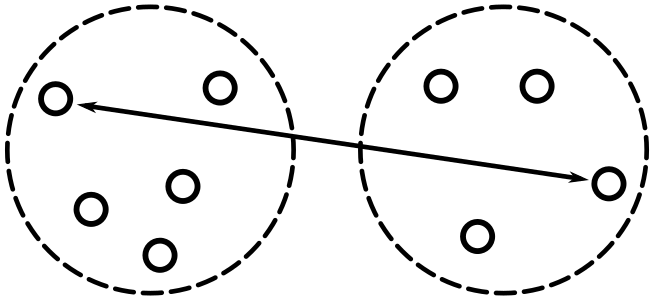
\includegraphics[width=.7\textwidth]{complete-link.png}
    \caption{Мера схожести кластеров по дальнему соседу.}
\end{figure}

Очевидным недостатком данной меры является то, что выбросы внутри кластера сильно влияют на конечный исход кластеризации \cite{zhao05}.

\subsubsection{По средней схожести}
Мера схожести кластеров можно определять как среднюю схожесть между новостями (Unweighted Pair Group Method with Arithmetic Mean, UPGMA):
\begin{equation} \label{eq:upgma}
    sim_{upgma}(C_i,C_j)=\frac{1}{|C_i||C_j|}\sum_{\mathbf{x}\in C_i}\sum_{\mathbf{y}\in C_j}sim(\vect{x},\vect{y})
\end{equation}

\subsubsection{По среднему в группе}
Данная мера известна как Group-Average Agglomerative Clustering (GAAC) и похожа на меру по средней схожести в том смысле, что определяется среднюю схожесть между новостями. Однако здесь учитываются все пары новостей, включая входящие в один кластер \cite{zhao05}:
\begin{equation}
    sim_{gaac}(C_i,C_j)=\frac{1}{(|C_i|+|C_j|)(|C_i|+|C_j|-1)}\sum_{x\in C}\sum_{\substack{y\in C,\\x\neq y}}\vect{x}\cdot\vect{y},
\end{equation}
где $C=C_i\cup C_j$.

\subsection{Методы кластеризации}
\subsubsection{k-средних}
Метод k-средних~--- наиболее популярный метод кластеризации. Данный алгоритм требует не только новости, но ещё и количество кластеров $k$.

Основная идея заключается в том, что на каждой итерации вычисляется центр масс для каждого кластера, полученного на предыдущем шаге, затем новости разбиваются на кластеры вновь в соответствии с тем, какой из новых центров оказался ближе по выбранной метрике к векторному представлению новости:
\begin{equation}
    \vect{C}(\Omega)=\frac{1}{|\Omega|}\sum_{x\in\Omega}\vect{x},
\end{equation}
\begin{conditions}
    $\vect{C}$ & новый центр кластера; \\
    $\Omega$ & множество новостей, входящих в кластер. \\
\end{conditions}

Алгоритм завершается, когда достигается критерий останова. Обычно в качестве такого критерия берут момент, когда между итерациями состав кластеров не поменялся. При этом можно показать, что процесс завершится за конечное число итерация и зацикливание невозможно \cite{manning09}.

\subsubsection{HAC}
Hierarchical Agglomerative Clustering (HAC)~--- алгоритм иерархической кластеризации с построением иерархии снизу вверх \cite{manning09}. Первоначально создаётся по кластеру на каждую новость, после чего на каждой итерации объединяются два наиболее схожих кластеров в один. Такая процедура повторяется до тех пор, пока не останется один единственный кластер, включающий в себя все остальные. В результате получаем дерево кластеров.

\subsubsection{Разделяющий метод k-средних}
Данный метод использует два типа кластеризации: иерархическую (сверху вниз) и разделяемую \cite{steinbach00}. Алгоритм начинает работу с создания одного кластера, включающего в себя все новости. Далее каждый кластер рекурсивно делится на $k$ кластеров методом k-средних, пока не будет достигнуто заданное количество кластеров или схожесть новостей внутри кластера не достигнет заданной константы.

\subsubsection{DHCA}
Развитием алгоритма HAC является Algorithm (DHCA) \cite{gil05}. Данные алгоритм является онлайновым, то есть обладает способностью обрабатывать новости по мере их поступления. Стоит отметить, что результат работы алгоритма не зависит от порядка обработки новостей.

Работа алгоритма начинается с создания для каждой новости кластера, после чего строится граф $\beta$-схожести (рис.~\ref{fig:beta-similarity}), где существуют рёбра только межу кластерами схожих более, чем на $\beta$. После чего для каждой вершины оставляется только связи с максимальной схожестью. Образованные компоненты связности и будут новыми кластерами (рис.~\ref{fig:max-similarity}). После чего процесс повторяется снова, причём в качестве меры схожести между кластерами используется UPGMA (\ref{eq:upgma}).

\begin{figure}
    \centering
    \begin{subfigure}{.5\textwidth}
        \centering
        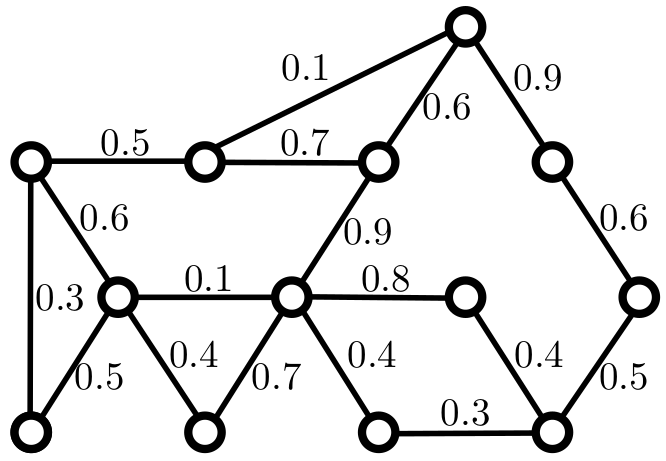
\includegraphics[width=.8\linewidth]{dhca-sim-graph.png}
        \caption{Граф $\beta$-схожести кластеров.}
        \label{fig:beta-similarity}
    \end{subfigure}%
    \begin{subfigure}{.5\textwidth}
        \centering
        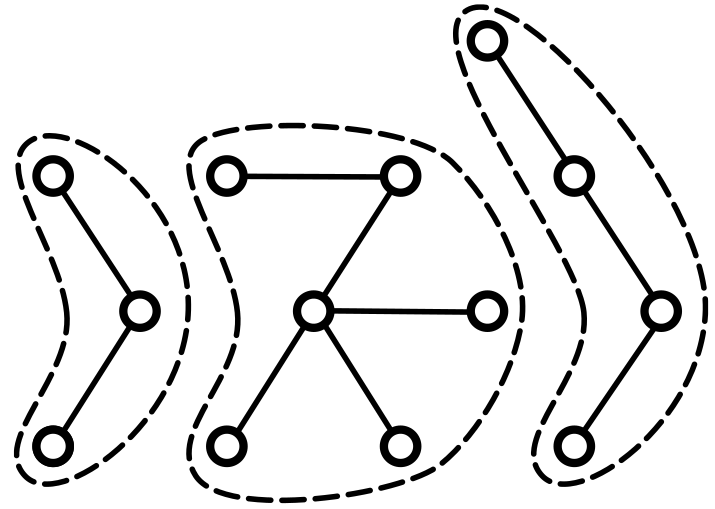
\includegraphics[width=.8\linewidth]{dhca-max-graph.png}
        \caption{Определение кластеров.}
        \label{fig:max-similarity}
    \end{subfigure}
    \caption{Пример работы DHCA.}
\end{figure}

\subsubsection{ICA}
Incremental Clustering Algorithm (ICA)~--- простой алгоритм кластеризации, позволяющий кластеризировать поток новостей \cite{lonnberg13}.

Для каждой поступающей новости находится ближайший кластер по методу UPGMA (\ref{eq:upgma}). Если схожесть с ближайшим кластером превышает заданный порог, то новость добавляется в кластер, иначе~--- создаётся новый кластер, содержащий только данную новость.

Существуют модификации данного алгоритма, позволяющие значительно сократить количество вычислений схожести кластеров \cite{lonnberg13} путём разбиения пространства кластеров.

\subsubsection{Выбор алгоритма кластеризации} \label{sssec:clustering-comparision}
Рассмотрим основные требования к алгоритму кластеризации согласно поставленной задачи:
\begin{enumerate}
    \item Алгоритм должен быть онлайновым, так как мы имеем дело с потоком новостей;
    \item В алгоритме не должно фиксироваться количество кластеров, так как каждая приходящая новость может образовывать новый сюжет, а значит и новый кластер;
    \item Должны существовать модификации алгоритма для оптимизации вычисления схожести кластеров.
\end{enumerate}

\begin{table}[ht]
    \centering
    \begin{tabular}{ l | c | c | c | c | >{\columncolor[gray]{0.8}} c }
        \hline
        & k-ср. & разд. k-ср. &  HAC & DHCA & ICA \\ \hline\hline
        Адаптивное кол-во кластеров & $-$ & $+$ & $+$ & $+$ & $+$ \\ \hline
        Иерархические кластеры      & $-$ & $+$ & $+$ & $+$ & $-$ \\ \hline
        Онлайновый алгоритм         & $-$ & $-$ & $-$ & $+$ & $+$ \\ \hline
        Возможность оптимизаций     & $+$ & $-$ & $-$ & $-$ & $+$ \\
        \hline
    \end{tabular}
    \caption{Сравнение алгоритмов кластеризации.}
    \label{tbl:clustering}
\end{table}

Исходя из требований к задаче и оценки алгоритмов (\ref{tbl:clustering}) имеет смысл выбрать ICA.

\section{Ранжирование источников}
Задача ранжирования источников по степени доверии к ним заключается в определении рейтинга источника по имеющейся оценке недостоверности новостей, публикуемых источником.

Рассмотрим несколько методов такого ранжирования.

\subsection{Простое ранжирование} \label{ssec:simple-ranking}
Поскольку публикация недостоверной новости должно вести к уменьшения рейтинга источника, то можно начислять штрафные очки каждый раз, когда источник публикует недостоверную новость, причём количество начисляемых очков пропорционально степени уверенности в недостоверности новости.

Таким образом, рейтинг источника $S$ за промежуток времени $t$ можно определить как
\begin{equation}
    score_S(t)=\sum_{x\in S(t)} p_x,
\end{equation}
где $p_x$~--- уверенность в недостоверности новости.

При таком определении менее достоверные источники получают выше рейтинг, чем более достоверные.

\subsection{Ссылочное ранжирование}
Для более сложного ранжирования можно использовать информацию о связи источника с другими источниками через новости. Для данного подхода недостаточно только информации о сюжетах, необходимо так же определять дубликаты и первоисточники.

Рассмотрим граф новостей (рис.~\ref{fig:news-graph}). В результате обнаружения дубликатов и объединения новостей в сюжеты, получаем множество связей между новостями, которые представляются тремя видами направленных рёбер:
\begin{enumerate}
    \item отношение <<дублирует>>;
    \item отношение <<схожий сюжет>>;
    \item отношение <<тематическое продолжение>>.
\end{enumerate}

С каждым ребром ставится в соответствие некоторое число, означающее силу связи.

\begin{figure}[h]
    \centering
    \begin{tikzpicture}[]
        \begin{scope}[every node/.style={circle,thick,draw}]
            \node (A) at (-3.5,0) {$A (0.8)$};
            \node (B) at (0,3.5) {$B (0.42)$};
            \node (C) at (1.5,1) {$C (?)$};
            \node (E) at (5.5,-2) {$E (0.6)$};
            \node (F) at (6,3) {$F (0.9)$};
        \end{scope}

        \begin{scope}[>={Stealth[black]},
                every node/.style={fill=white,circle},
            every edge/.style={draw=gray,very thick}]
            \path[->] (A) edge node {$0.2$} (C);
            \path[->] (E) edge node {$0.3$} (C);
            \path[->] (F) edge node {$0.3$} (C);
            \path[->] (A) edge (B);
            \path[->] (A) edge (E);
            \path[->] (B) edge (F);
            \path[->] (E) edge (F);
            \path[->] (F) edge[bend left=40] (E);
            \path[<-] (E) edge ++(2,0);
            \path[->] (A) edge ++(0,-2);
            \path[<-] (A) edge ++(-2.3,0);
            \path[->] (F) edge ++(2,0);
            \path[<-] (F) edge ++(0,2);
            \path[<-] (B) edge ++(-3,0);
        \end{scope}
    \end{tikzpicture}
    \caption{Граф новостей}
    \label{fig:news-graph}
\end{figure}

Поскольку каждая новость так же связана с источником, из которого получена данная новость, то мы можем перейти к схожему графу для источников. Теперь, если пометить некоторую новость как фальсифицированную, то мы можем, используя установленные связи, передать часть веса остальным новостям, связанных с данной, а значит и источнику, связанному с данной новостью.

В качестве алгоритма распространения веса могут быть использованы модификации PageRank или HITS алгоритмов \cite{segaran07}.

Из-за большей сложности (требуется так же определять дубликаты и первоисточники новостей) данный метод в работе не используется.

